
\section{1A2 MOE Models}

\begin{table}[H]
\caption{1A2 MOE Model Results}
\begin{minipage}{.5\linewidth}
\centering
\begin{tabular}{|l|l|l|l|}
\hline
\multicolumn{4}{|c|}{1A2 Training Set Accuracy}   \\ \hline
PC & Total          & Active          & Inactive  \\ \hline
2  & 0.638          & 0.752           & 0.522     \\ \hline
5  & 0.704          & 0.746           & 0.662     \\ \hline
10 & 0.734          & 0.755           & 0.712     \\ \hline
15 & 0.737          & 0.770           & 0.704     \\ \hline
20 & 0.741          & 0.781           & 0.701     \\ \hline
30 & 0.735          & 0.782           & 0.686     \\ \hline
44 & 0.725          & 0.777           & 0.672     \\ \hline
\end{tabular}
\end{minipage}
\begin{minipage}{.5\linewidth}
\centering
\begin{tabular}{|l|l|l|l|}
\hline
\multicolumn{4}{|c|}{1A2 Test Set Accuracy}     \\ \hline
PC & Total          & Active          & Inactive \\ \hline
2  & 0.632          & 0.758           & 0.517   \\ \hline
5  & 0.705          & 0.773           & 0.643   \\ \hline
10 & 0.746          & 0.749           & 0.743   \\ \hline
15 & 0.752          & 0.775           & 0.731   \\ \hline
20 & 0.748          & 0.779           & 0.721   \\ \hline
30 & 0.739          & 0.783           & 0.698   \\ \hline
44 & 0.720          & 0.773           & 0.672   \\ \hline
\end{tabular}
\end{minipage}
\end{table}

The 1A2 models were trained on 4820 inhibitors and 4780 non-inhibitors and tested on 1180 inhibitors and 1220 non-inhibitors.
\begin{figure}[H]
\includegraphics[width=1\textwidth]{../img/1a2_moe_model_accuracy.png}
\caption{1A2 MOE Model Accuracy}
\label{fig:1a2}
\end{figure}

With 20 principal components (Figure~\ref{fig:1a2}), test set accuracy is 0.748 overall, 0.779 on inhibitors and 0.721 on non-inhibitors.


\section{2C9 MOE Models}

\begin{table}[H]
\caption{2C9 MOE Model Results}
\begin{minipage}{.5\linewidth}
\centering
\begin{tabular}{|l|l|l|l|}
\hline
\multicolumn{4}{|c|}{2C9 Training Set Accuracy} \\ \hline
PC & Total          & Active          & Inactive\\ \hline
2  & 0.620          & 0.695           & 0.547   \\ \hline
5  & 0.683          & 0.722           & 0.645   \\ \hline
10 & 0.699          & 0.744           & 0.655   \\ \hline
15 & 0.702          & 0.752           & 0.653   \\ \hline
20 & 0.710          & 0.756           & 0.665   \\ \hline
30 & 0.711          & 0.754           & 0.668   \\ \hline
44 & 0.712          & 0.770           & 0.655   \\ \hline
\end{tabular}
\end{minipage}
\begin{minipage}{.5\linewidth}
\centering
\begin{tabular}{|l|l|l|l|}
\hline
\multicolumn{4}{|c|}{2C9 Test Set Accuracy}     \\ \hline
PC & Total          & Active          & Inactive\\ \hline
2  & 0.609          & 0.702           & 0.510   \\ \hline
5  & 0.675          & 0.713           & 0.634   \\ \hline
10 & 0.682          & 0.730           & 0.632   \\ \hline
15 & 0.686          & 0.739           & 0.630   \\ \hline
20 & 0.685          & 0.731           & 0.636   \\ \hline
30 & 0.690          & 0.730           & 0.646   \\ \hline
44 & 0.688          & 0.750           & 0.621   \\ \hline
\end{tabular}
\end{minipage}
\end{table}

The 2C9 models were trained on 3266 inhibitors and 3327 non-inhibitors and tested on 855 inhibitors and 794 non-inhibitors.
\begin{figure}[H]
\includegraphics[width=1\textwidth]{../img/2c9_moe_model_accuracy.png}
\caption{2C9 MOE Model Accuracy}
\label{fig:2c9}
\end{figure}

With 20 principal components (Figure~\ref{fig:2c9}), test set accuracy is 0.685 overall, 0.731 on inhibitors and 0.636 on non-inhibitors.


\section{2C19 MOE Models}

\begin{table}[H]
\caption{2C19 MOE Model Results}
\begin{minipage}{.5\linewidth}
\centering
\begin{tabular}{|l|l|l|l|}
\hline
\multicolumn{4}{|c|}{2C19 Training Set Accuracy} \\ \hline
PC & Total          & Active          & Inactive \\ \hline
2  & 0.585          & 0.774           & 0.396   \\ \hline
5  & 0.685          & 0.726           & 0.645   \\ \hline
10 & 0.699          & 0.736           & 0.661    \\ \hline
15 & 0.700          & 0.747           & 0.653    \\ \hline
20 & 0.705          & 0.749           & 0.661    \\ \hline
30 & 0.717          & 0.761           & 0.672    \\ \hline
44 & 0.708          & 0.777           & 0.640    \\ \hline
\end{tabular}
\end{minipage}%
\begin{minipage}{.5\linewidth}
\centering
\begin{tabular}{|l|l|l|l|}
\hline
\multicolumn{4}{|c|}{2C19 Test Set Accuracy}       \\ \hline
PC & Total          & Active          & Inactive   \\ \hline
2  & 0.593          & 0.775           & 0.408      \\ \hline
5  & 0.683          & 0.729           & 0.635      \\ \hline
10 & 0.691          & 0.731           & 0.650      \\ \hline
15 & 0.687          & 0.736           & 0.637      \\ \hline
20 & 0.698          & 0.758           & 0.638      \\ \hline
30 & 0.699          & 0.764           & 0.633      \\ \hline
44 & 0.694          & 0.774           & 0.613      \\ \hline
\end{tabular}
\end{minipage}
\end{table}

The 2C19 models were trained on 4721 inhibitors and 4741 non-inhibitors and tested on 1193 inhibitors and 1173 non-inhibitors.
\begin{figure}[H]
\includegraphics[width=1\textwidth]{../img/2c19_moe_model_accuracy.png}
\caption{2C19 MOE Model Accuracy}
\label{fig:2c19}
\end{figure}

With 20 principal components (Figure~\ref{fig:2c19}), test set accuracy is 0.698 overall, 0.758 on inhibitors and 0.638 on non-inhibitors.


\section{2D6 MOE Models}

\begin{table}[H]
\caption{2D6 MOE Model Results}
\begin{minipage}{.5\linewidth}
\centering
\begin{tabular}{|l|l|l|l|}
\hline
\multicolumn{4}{|c|}{2D6 Training Set Accuracy} \\ \hline
PC & Total          & Active          & Inactive\\ \hline
2  & 0.589          & 0.753           & 0.426   \\ \hline
5  & 0.670          & 0.706           & 0.634   \\ \hline
10 & 0.685          & 0.721           & 0.648   \\ \hline
15 & 0.686          & 0.709           & 0.662   \\ \hline
20 & 0.705          & 0.721           & 0.689   \\ \hline
30 & 0.703          & 0.732           & 0.673   \\ \hline
44 & 0.690          & 0.725           & 0.656   \\ \hline
\end{tabular}
\end{minipage}
\begin{minipage}{.5\linewidth}
\centering
\begin{tabular}{|l|l|l|l|}
\hline
\multicolumn{4}{|c|}{2D6 Test Set Accuracy}      \\ \hline
PC & Total          & Active          & Inactive \\ \hline
2  & 0.590          & 0.738           & 0.443    \\ \hline
5  & 0.667          & 0.685           & 0.650    \\ \hline
10 & 0.662          & 0.688           & 0.636    \\ \hline
15 & 0.665          & 0.692           & 0.639    \\ \hline
20 & 0.683          & 0.699           & 0.668    \\ \hline
30 & 0.686          & 0.696           & 0.677    \\ \hline
44 & 0.669          & 0.707           & 0.632    \\ \hline
\end{tabular}
\end{minipage}
\end{table}

The 2D6 models were trained on 2219 inhibitors and 2214 non-inhibitors and tested on 552 inhibitors and 557 non-inhibitors.
\begin{figure}[H]
\includegraphics[width=1\textwidth]{../img/2d6_moe_model_accuracy.png}
\caption{2D6 MOE Model Accuracy}
\label{fig:2d6}
\end{figure}

With 20 principal components (Figure~\ref{fig:2d6}), test set accuracy is 0.683 overall, 0.699 on inhibitors and 0.668 on non-inhibitors.


\section{3A4 MOE Models}

\begin{table}[H]
\caption{3A4 MOE Model Results}
\begin{minipage}{.5\linewidth}
\centering
\begin{tabular}{|l|l|l|l|}
\hline
\multicolumn{4}{|c|}{3A4 Training Set Accuracy} \\ \hline
PC & Total          & Active          & Inactive \\ \hline
2  & 0.644          & 0.699           & 0.589   \\ \hline
5  & 0.675          & 0.727           & 0.623   \\ \hline
10 & 0.698          & 0.741           & 0.655   \\ \hline
15 & 0.701          & 0.746           & 0.656   \\ \hline
20 & 0.705          & 0.749           & 0.660   \\ \hline
30 & 0.709          & 0.761           & 0.657   \\ \hline
44 & 0.698          & 0.773           & 0.623   \\ \hline
\end{tabular}
\end{minipage}
\begin{minipage}{.5\linewidth}
\centering
\begin{tabular}{|l|l|l|l|}
\hline
\multicolumn{4}{|c|}{3A4 Test Set Accuracy}      \\ \hline
PC & Total          & Active          & Inactive \\ \hline
2  & 0.627          & 0.683           & 0.573    \\ \hline
5  & 0.656          & 0.719           & 0.595    \\ \hline
10 & 0.677          & 0.719           & 0.637    \\ \hline
15 & 0.680          & 0.733           & 0.628    \\ \hline
20 & 0.686          & 0.736           & 0.638    \\ \hline
30 & 0.686          & 0.742           & 0.631    \\ \hline
44 & 0.676          & 0.747           & 0.607    \\ \hline
\end{tabular}
\end{minipage}
\end{table}

The 3A4 models were trained on 4234 inhibitors and 4193 non-inhibitors and tested on 1033 inhibitors and 1074 non-inhibitors.
\begin{figure}[H]
\includegraphics[width=1\textwidth]{../img/3a4_moe_model_accuracy.png}
\caption{3A4 MOE Model Accuracy}
\label{fig:3a4}
\end{figure}

With 20 principal components (Figure~\ref{fig:3a4}), test set accuracy is 0.686 overall, 0.736 on inhibitors and 0.638 on non-inhibitors.


\section{1A2 Classification Method Comparison}

\begin{table}[H]
\caption[Comparison of Classification Methods for 1A2]{Comparison of Classification Methods for 1A2. Python training accuracies are 5-fold cross-validation estimates.}
\centering
\begin{tabular}{|l|l|l|}
\hline
\multicolumn{3}{|c|}{1A2 Classification Method Comparison} \\ \hline
          & Training Set & Test Set \\ \hline
MOE 20PC  & 0.741        & 0.748    \\ \hline
\textit{k}-NN    & 0.765        & 0.780    \\ \hline
Random Forest & 0.775    & 0.792    \\ \hline
SVM       & 0.798        & 0.808    \\ \hline
\end{tabular}
\end{table}

On the 1A2 test set, MOE Binary QSAR with 20 principal components reached an accuracy of 0.748, compared with 0.780 for \textit{k}-NN, 0.792 for random forest and 0.808 for SVM.

\section{2C9 Classification Method Comparison}

\begin{table}[H]
\caption[Comparison of Classification Methods for 2C9]{Comparison of Classification Methods for 2C9. Python training accuracies are 5-fold cross-validation estimates.}
\centering
\begin{tabular}{|l|l|l|}
\hline
\multicolumn{3}{|c|}{2C9 Classification Method Comparison} \\ \hline
          & Training Set & Test Set \\ \hline
MOE 20PC  & 0.710        & 0.685    \\ \hline
\textit{k}-NN    & 0.719        & 0.712    \\ \hline
Random Forest & 0.725    & 0.725    \\ \hline
SVM       & 0.748        & 0.754    \\ \hline
\end{tabular}
\end{table}

On the 2C9 test set, MOE Binary QSAR with 20 principal components reached an accuracy of 0.685, compared with 0.712 for \textit{k}-NN, 0.725 for random forest and 0.754 for SVM.

\section{2C19 Classification Method Comparison}

\begin{table}[H]
\caption[Comparison of Classification Methods for 2C19]{Comparison of Classification Methods for 2C19. Python training accuracies are 5-fold cross-validation estimates.}
\centering
\begin{tabular}{|l|l|l|}
\hline
\multicolumn{3}{|c|}{2C19 Classification Method Comparison} \\ \hline
          & Training Set & Test Set \\ \hline
MOE 20PC  & 0.705        & 0.698    \\ \hline
\textit{k}-NN    & 0.731        & 0.746    \\ \hline
Random Forest & 0.734    & 0.733    \\ \hline
SVM       & 0.764        & 0.780    \\ \hline
\end{tabular}
\end{table}

On the 2C19 test set, MOE Binary QSAR with 20 principal components reached an accuracy of 0.698, compared with 0.746 for \textit{k}-NN, 0.733 for random forest and 0.780 for SVM.

\section{2D6 Classification Method Comparison}

\begin{table}[H]
\caption[Comparison of Classification Methods for 2D6]{Comparison of Classification Methods for 2D6. Python training accuracies are 5-fold cross-validation estimates.}
\centering
\begin{tabular}{|l|l|l|}
\hline
\multicolumn{3}{|c|}{2D6 Classification Method Comparison} \\ \hline
          & Training Set & Test Set \\ \hline
MOE 20PC  & 0.705        & 0.683    \\ \hline
\textit{k}-NN    & 0.717        & 0.718    \\ \hline
Random Forest & 0.728    & 0.729    \\ \hline
SVM       & 0.759        & 0.752    \\ \hline
\end{tabular}
\end{table}

On the 2D6 test set, MOE Binary QSAR with 20 principal components reached an accuracy of 0.683, compared with 0.718 for \textit{k}-NN, 0.729 for random forest and 0.752 for SVM.


\section{3A4 Classification Method Comparison}

\begin{table}[H]
\caption[Comparison of Classification Methods for 3A4]{Comparison of Classification Methods for 3A4. Python training accuracies are 5-fold cross-validation estimates.}
\centering
\begin{tabular}{|l|l|l|}
\hline
\multicolumn{3}{|c|}{3A4 Classification Method Comparison} \\ \hline
          & Training Set & Test Set \\ \hline
MOE 20PC  & 0.705        & 0.686    \\ \hline
\textit{k}-NN    & 0.714        & 0.704    \\ \hline
Random Forest & 0.718    & 0.728    \\ \hline
SVM       & 0.754        & 0.746    \\ \hline
\end{tabular}
\end{table}

On the 3A4 test set, MOE Binary QSAR with 20 principal components reached an accuracy of 0.686, compared with 0.704 for \textit{k}-NN, 0.728 for random forest and 0.746 for SVM.


\section{Python Classifier Test Set Results}\label{sec:pytest}

\begin{table}[H]
\caption{Python Classifier Test Set Results}
\centering
\begin{tabular}{|l|l|l|l|l|l|}
\hline
Isozyme & Method & Accuracy & TPR & TNR & AUC \\ \hline
\multirow{3}{*}{1A2} & \textit{k}-NN & 0.780 & 0.825 & 0.737 & 0.852 \\ \cline{2-6}
 & Random Forest & 0.792 & 0.775 & 0.808 & 0.866 \\ \cline{2-6}
 & SVM & 0.808 & 0.849 & 0.768 & 0.886 \\ \hline
\multirow{3}{*}{2C9} & \textit{k}-NN & 0.712 & 0.749 & 0.673 & 0.771 \\ \cline{2-6}
 & Random Forest & 0.725 & 0.705 & 0.746 & 0.791 \\ \cline{2-6}
 & SVM & 0.754 & 0.806 & 0.698 & 0.816 \\ \hline
\multirow{3}{*}{2C19} & \textit{k}-NN & 0.746 & 0.786 & 0.705 & 0.803 \\ \cline{2-6}
 & Random Forest & 0.733 & 0.724 & 0.742 & 0.807 \\ \cline{2-6}
 & SVM & 0.780 & 0.837 & 0.723 & 0.845 \\ \hline
\multirow{3}{*}{2D6} & \textit{k}-NN & 0.718 & 0.746 & 0.689 & 0.780 \\ \cline{2-6}
 & Random Forest & 0.729 & 0.649 & 0.808 & 0.795 \\ \cline{2-6}
 & SVM & 0.752 & 0.726 & 0.777 & 0.830 \\ \hline
\multirow{3}{*}{3A4} & \textit{k}-NN & 0.704 & 0.749 & 0.660 & 0.771 \\ \cline{2-6}
 & Random Forest & 0.728 & 0.694 & 0.761 & 0.815 \\ \cline{2-6}
 & SVM & 0.746 & 0.802 & 0.692 & 0.831 \\ \hline
\end{tabular}
\end{table}

TPR is the fraction of actual inhibitors predicted correctly, TNR the fraction of actual non-inhibitors predicted correctly, and AUC the area under the receiver operating characteristic curve. \textit{k}-NN and SVM were more accurate on inhibitors than on non-inhibitors for most isozymes, whereas random forest was consistently more accurate on non-inhibitors.

\section{Overall Method Comparison}

\begin{figure}[H]
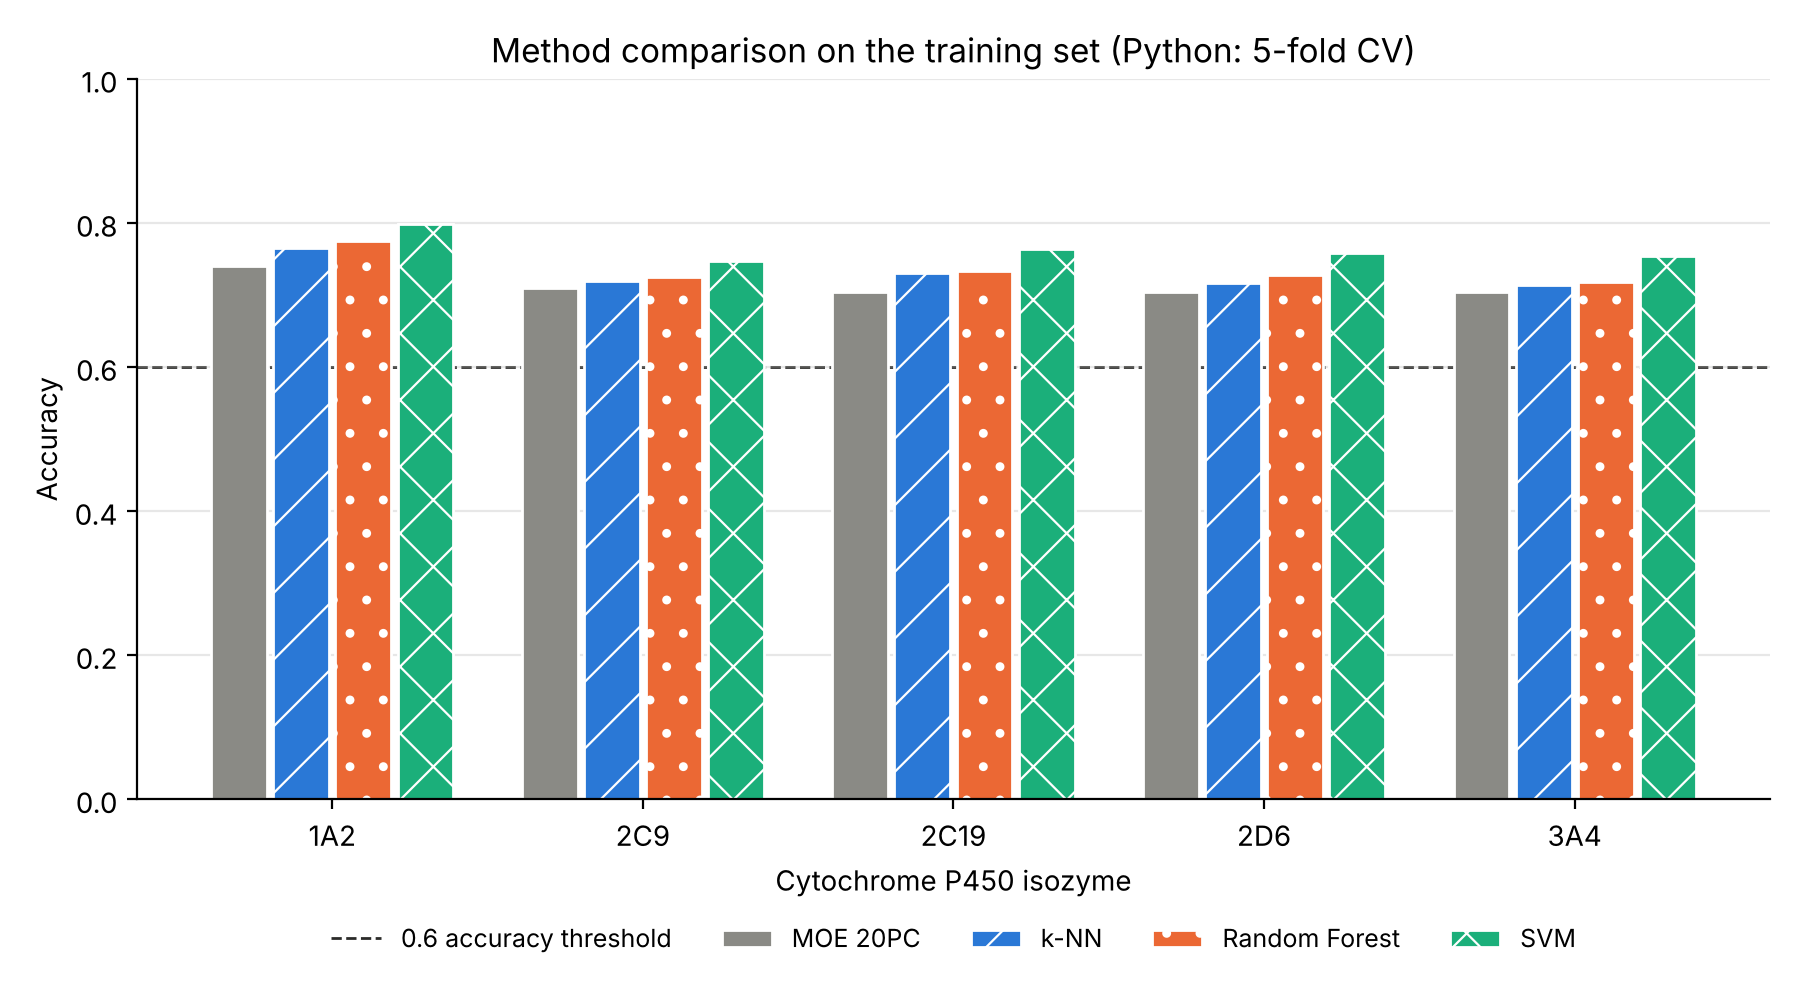
\includegraphics[width=1\textwidth]{../img/method_comparison_training_set.png}
\caption{Inhibitor Classification Method Comparison on the Training Set}
\end{figure}

On the training set (cross-validated for the Python classifiers), all three Python classifiers matched or exceeded MOE Binary QSAR for every isozyme, and the support vector machine classifier had the highest accuracy in each case.

\begin{figure}[H]
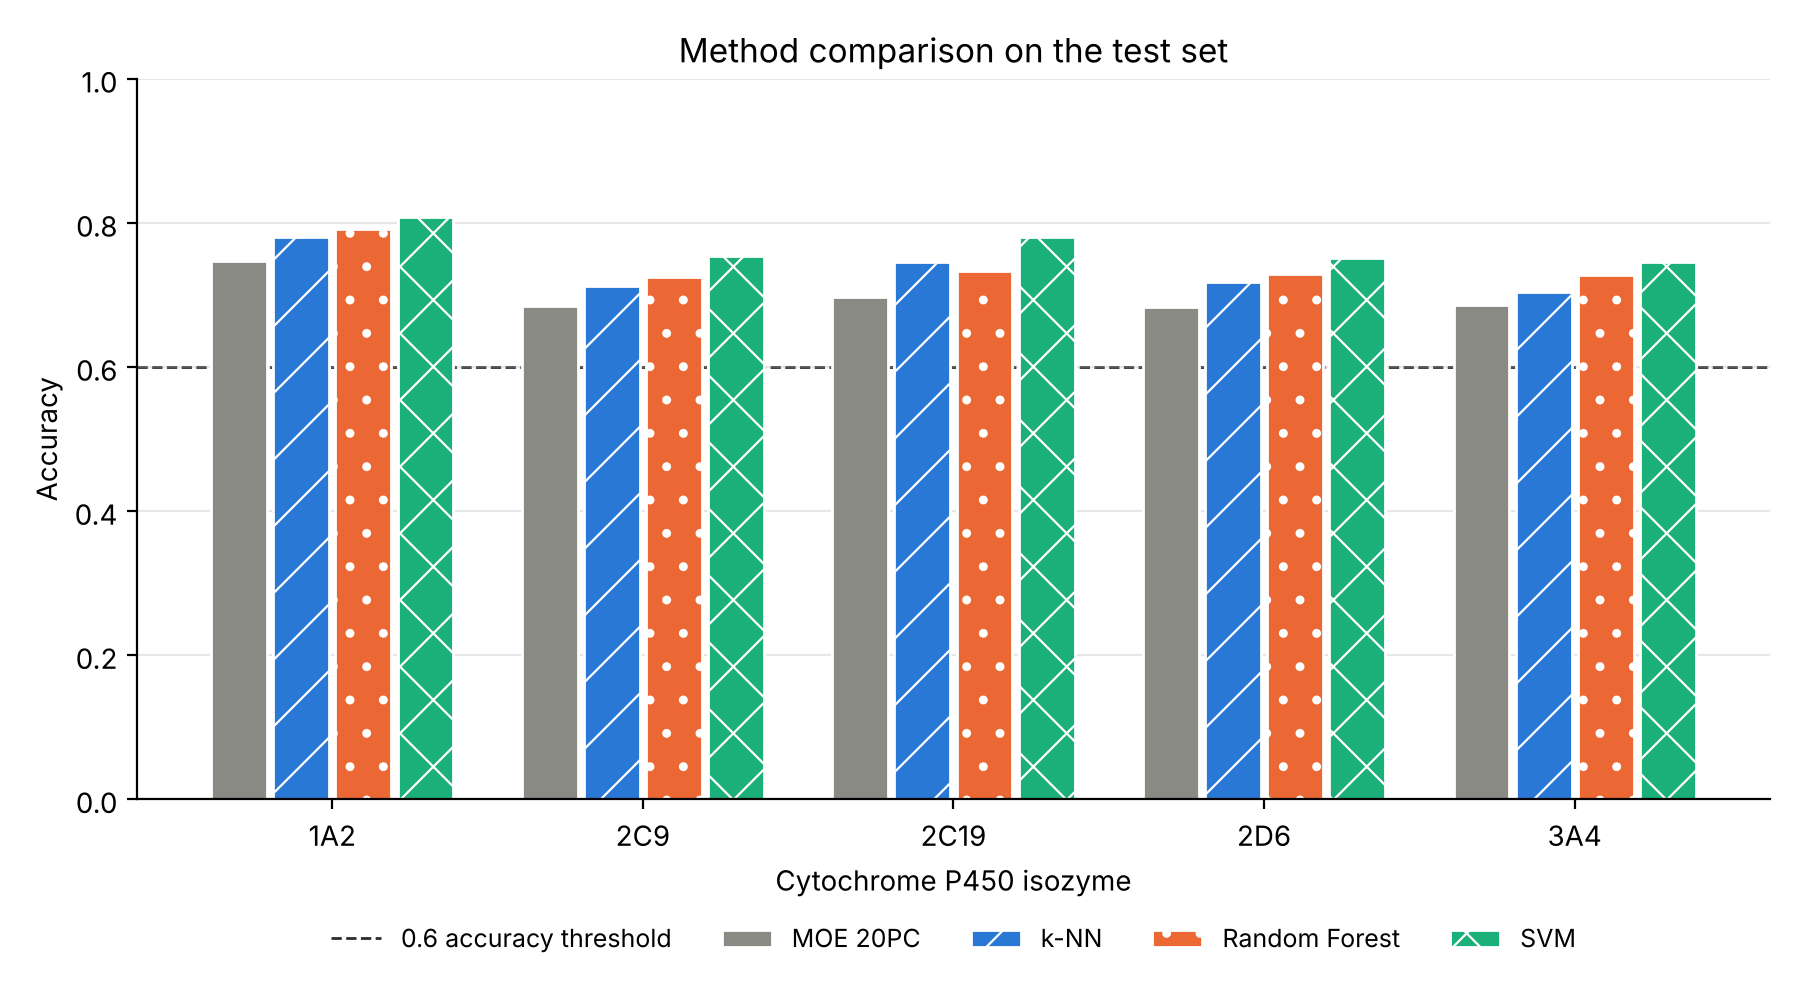
\includegraphics[width=1\textwidth]{../img/method_comparison_test_set.png}
\caption{Inhibitor Classification Method Comparison on the Test Set}
\end{figure}

On the test set, all three Python classifiers exceeded MOE Binary QSAR for every isozyme, and the support vector machine classifier had the highest accuracy in each case.




